%%%%%%%%%%%%%%%%%%%%%%%%%%%%%%%%%%%%%%%%%%%%%%%%%%%%%%%%%%%%%%%
%% OXFORD THESIS TEMPLATE

% Use this template to produce a standard thesis that meets the Oxford University requirements for DPhil submission
%
% Originally by Keith A. Gillow (gillow@maths.ox.ac.uk), 1997
% Modified by Sam Evans (sam@samuelevansresearch.org), 2007
% Modified by John McManigle (john@oxfordechoes.com), 2015
% Modified by Ulrik Lyngs (ulrik.lyngs@cs.ox.ac.uk), 2018, for use with R Markdown
%
% Ulrik Lyngs, 25 Nov 2018: Following John McManigle, broad permissions are granted to use, modify, and distribute this software
% as specified in the MIT License included in this distribution's LICENSE file.
%
% John tried to comment this file extensively, so read through it to see how to use the various options.  Remember
% that in LaTeX, any line starting with a % is NOT executed.  Several places below, you have a choice of which line to use
% out of multiple options (eg draft vs final, for PDF vs for binding, etc.)  When you pick one, add a % to the beginning of
% the lines you don't want.


%%%%% CHOOSE PAGE LAYOUT
% The most common choices should be below.  You can also do other things, like replacing "a4paper" with "letterpaper", etc.

% This one will format for two-sided binding (ie left and right pages have mirror margins; blank pages inserted where needed):
%\documentclass[a4paper,twoside]{templates/ociamthesis}
% This one will format for one-sided binding (ie left margin > right margin; no extra blank pages):
%\documentclass[a4paper]{ociamthesis}
% This one will format for PDF output (ie equal margins, no extra blank pages):
%\documentclass[a4paper,nobind]{templates/ociamthesis}
%UL 2 Dec 2018: pass this in from YAML
\documentclass[a4paper, nobind]{templates/ociamthesis}


% UL 30 Nov 2018 pandoc puts lists in 'tightlist' command when no space between bullet points in Rmd file
\providecommand{\tightlist}{%
  \setlength{\itemsep}{0pt}\setlength{\parskip}{0pt}}
 
% UL 1 Dec 2018, fix to include code in shaded environments
\usepackage{color}
\usepackage{fancyvrb}
\newcommand{\VerbBar}{|}
\newcommand{\VERB}{\Verb[commandchars=\\\{\}]}
\DefineVerbatimEnvironment{Highlighting}{Verbatim}{commandchars=\\\{\}}
% Add ',fontsize=\small' for more characters per line
\usepackage{framed}
\definecolor{shadecolor}{RGB}{248,248,248}
\newenvironment{Shaded}{\begin{snugshade}}{\end{snugshade}}
\newcommand{\AlertTok}[1]{\textcolor[rgb]{0.94,0.16,0.16}{#1}}
\newcommand{\AnnotationTok}[1]{\textcolor[rgb]{0.56,0.35,0.01}{\textbf{\textit{#1}}}}
\newcommand{\AttributeTok}[1]{\textcolor[rgb]{0.77,0.63,0.00}{#1}}
\newcommand{\BaseNTok}[1]{\textcolor[rgb]{0.00,0.00,0.81}{#1}}
\newcommand{\BuiltInTok}[1]{#1}
\newcommand{\CharTok}[1]{\textcolor[rgb]{0.31,0.60,0.02}{#1}}
\newcommand{\CommentTok}[1]{\textcolor[rgb]{0.56,0.35,0.01}{\textit{#1}}}
\newcommand{\CommentVarTok}[1]{\textcolor[rgb]{0.56,0.35,0.01}{\textbf{\textit{#1}}}}
\newcommand{\ConstantTok}[1]{\textcolor[rgb]{0.00,0.00,0.00}{#1}}
\newcommand{\ControlFlowTok}[1]{\textcolor[rgb]{0.13,0.29,0.53}{\textbf{#1}}}
\newcommand{\DataTypeTok}[1]{\textcolor[rgb]{0.13,0.29,0.53}{#1}}
\newcommand{\DecValTok}[1]{\textcolor[rgb]{0.00,0.00,0.81}{#1}}
\newcommand{\DocumentationTok}[1]{\textcolor[rgb]{0.56,0.35,0.01}{\textbf{\textit{#1}}}}
\newcommand{\ErrorTok}[1]{\textcolor[rgb]{0.64,0.00,0.00}{\textbf{#1}}}
\newcommand{\ExtensionTok}[1]{#1}
\newcommand{\FloatTok}[1]{\textcolor[rgb]{0.00,0.00,0.81}{#1}}
\newcommand{\FunctionTok}[1]{\textcolor[rgb]{0.00,0.00,0.00}{#1}}
\newcommand{\ImportTok}[1]{#1}
\newcommand{\InformationTok}[1]{\textcolor[rgb]{0.56,0.35,0.01}{\textbf{\textit{#1}}}}
\newcommand{\KeywordTok}[1]{\textcolor[rgb]{0.13,0.29,0.53}{\textbf{#1}}}
\newcommand{\NormalTok}[1]{#1}
\newcommand{\OperatorTok}[1]{\textcolor[rgb]{0.81,0.36,0.00}{\textbf{#1}}}
\newcommand{\OtherTok}[1]{\textcolor[rgb]{0.56,0.35,0.01}{#1}}
\newcommand{\PreprocessorTok}[1]{\textcolor[rgb]{0.56,0.35,0.01}{\textit{#1}}}
\newcommand{\RegionMarkerTok}[1]{#1}
\newcommand{\SpecialCharTok}[1]{\textcolor[rgb]{0.00,0.00,0.00}{#1}}
\newcommand{\SpecialStringTok}[1]{\textcolor[rgb]{0.31,0.60,0.02}{#1}}
\newcommand{\StringTok}[1]{\textcolor[rgb]{0.31,0.60,0.02}{#1}}
\newcommand{\VariableTok}[1]{\textcolor[rgb]{0.00,0.00,0.00}{#1}}
\newcommand{\VerbatimStringTok}[1]{\textcolor[rgb]{0.31,0.60,0.02}{#1}}
\newcommand{\WarningTok}[1]{\textcolor[rgb]{0.56,0.35,0.01}{\textbf{\textit{#1}}}}
%UL 2 Dec 2018 add a bit of white space before and after code blocks
\renewenvironment{Shaded}
{
  \vspace{4pt}%
  \begin{snugshade}%
}{%
  \end{snugshade}%
  \vspace{4pt}%
}

%UL 2 Dec 2018 reduce whitespace around verbatim environments
\usepackage{etoolbox}
\makeatletter
\preto{\@verbatim}{\topsep=0pt \partopsep=0pt }
\makeatother

%UL 26 Mar 2019, enable strikethrough
\usepackage[normalem]{ulem}

%UL 15 Oct 2019, enable link highlighting to be turned off from YAML
\usepackage[colorlinks=false,pdfpagelabels,hidelinks=true]{hyperref}

%%%%% SELECT YOUR DRAFT OPTIONS
% Three options going on here; use in any combination.  But remember to turn the first two off before
% generating a PDF to send to the printer!

% This adds a "DRAFT" footer to every normal page.  (The first page of each chapter is not a "normal" page.)

% This highlights (in blue) corrections marked with (for words) \mccorrect{blah} or (for whole
% paragraphs) \begin{mccorrection} . . . \end{mccorrection}.  This can be useful for sending a PDF of
% your corrected thesis to your examiners for review.  Turn it off, and the blue disappears.
\correctionstrue

%%%%% BIBLIOGRAPHY SETUP
% Note that your bibliography will require some tweaking depending on your department, preferred format, etc.
% The options included below are just very basic "sciencey" and "humanitiesey" options to get started.
% If you've not used LaTeX before, I recommend reading a little about biblatex/biber and getting started with it.
% If you're already a LaTeX pro and are used to natbib or something, modify as necessary.
% Either way, you'll have to choose and configure an appropriate bibliography format...

% The science-type option: numerical in-text citation with references in order of appearance.
% \usepackage[style=numeric-comp, sorting=none, backend=biber, doi=false, isbn=false]{biblatex}
% \newcommand*{\bibtitle}{References}

% The humanities-type option: author-year in-text citation with an alphabetical works cited.
% \usepackage[style=authoryear, sorting=nyt, backend=biber, maxcitenames=2, useprefix, doi=false, isbn=false]{biblatex}
% \newcommand*{\bibtitle}{Works Cited}

%UL 3 Dec 2018: set this from YAML in index.Rmd
\usepackage[style=authoryear, sorting=nyt, backend=biber, maxcitenames=2, useprefix, doi=true, isbn=false, uniquename=false]{biblatex}
\newcommand*{\bibtitle}{Works Cited}

% This makes the bibliography left-aligned (not 'justified') and slightly smaller font.
\renewcommand*{\bibfont}{\raggedright\small}

% Change this to the name of your .bib file (usually exported from a citation manager like Zotero or EndNote).
\addbibresource{references.bib}


% Uncomment this if you want equation numbers per section (2.3.12), instead of per chapter (2.18):
%\numberwithin{equation}{subsection}


%%%%% THESIS / TITLE PAGE INFORMATION
% Everybody needs to complete the following:
\title{Analyzing the Feature Importance of Different Variables on the Price of Ikea Products}
\author{Philip Krück, Johannes Pein}
\college{}

% Master's candidates who require the alternate title page (with candidate number and word count)
% must also un-comment and complete the following three lines:
%\masterssubmissiontrue
%\candidateno{933516}
%\wordcount{28,815}

% Uncomment the following line if your degree also includes exams (eg most masters):
%\renewcommand{\submittedtext}{Submitted in partial completion of the}
% Your full degree name.  (But remember that DPhils aren't "in" anything.  They're just DPhils.)
\degree{B.Sc. Business Informatics (18A-BI)}
% Term and year of submission, or date if your board requires (eg most masters)
\degreedate{04.12.2020}


%%%%% YOUR OWN PERSONAL MACROS
% This is a good place to dump your own LaTeX macros as they come up.
\modulename{Digital Toolbox: Data Business}
\lecturer{Lecturer: Ulf Köther}
\groupnumber{Group Number: 7}
\matriculationnumbers{Matriculation Numbers: 3938 (P.Krück), 4001 (J.Pein)}


% To make text superscripts shortcuts
	\renewcommand{\th}{\textsuperscript{th}} % ex: I won 4\th place
	\newcommand{\nd}{\textsuperscript{nd}}
	\renewcommand{\st}{\textsuperscript{st}}
	\newcommand{\rd}{\textsuperscript{rd}}

%%%%% THE ACTUAL DOCUMENT STARTS HERE
\begin{document}

%%%%% CHOOSE YOUR LINE SPACING HERE
% This is the official option.  Use it for your submission copy and library copy:
\setlength{\textbaselineskip}{22pt plus2pt}
% This is closer spacing (about 1.5-spaced) that you might prefer for your personal copies:
%\setlength{\textbaselineskip}{18pt plus2pt minus1pt}

% You can set the spacing here for the roman-numbered pages (acknowledgements, table of contents, etc.)
\setlength{\frontmatterbaselineskip}{17pt plus1pt minus1pt}


% UL: You can set the general paragraph spacing here - I've set it to 2pt (was 0) so
% it's less claustrophobic
\setlength{\parskip}{2pt plus 1pt}


% Leave this line alone; it gets things started for the real document.
\setlength{\baselineskip}{\textbaselineskip}


%%%%% CHOOSE YOUR SECTION NUMBERING DEPTH HERE
% You have two choices.  First, how far down are sections numbered?  (Below that, they're named but
% don't get numbers.)  Second, what level of section appears in the table of contents?  These don't have
% to match: you can have numbered sections that don't show up in the ToC, or unnumbered sections that
% do.  Throughout, 0 = chapter; 1 = section; 2 = subsection; 3 = subsubsection, 4 = paragraph...

% The level that gets a number:
\setcounter{secnumdepth}{2}
% The level that shows up in the ToC:
\setcounter{tocdepth}{2}


% JEM: Pages are roman numbered from here, though page numbers are invisible until ToC.  This is in
% keeping with most typesetting conventions.
\begin{romanpages}

% Title page is created here
\maketitle

%%%%% MINI TABLES
% This lays the groundwork for per-chapter, mini tables of contents.  Comment the following line
% (and remove \minitoc from the chapter files) if you don't want this.  Un-comment either of the
% next two lines if you want a per-chapter list of figures or tables.
  \dominitoc % include a mini table of contents

% This aligns the bottom of the text of each page.  It generally makes things look better.
\flushbottom

% This is where the whole-document ToC appears:
\tableofcontents

%%%%% LIST OF ABBREVIATIONS
% This example includes a list of abbreviations.  Look at text/abbreviations.tex to see how that file is
% formatted.  The template can handle any kind of list though, so this might be a good place for a
% glossary, etc.
% First parameter can be changed eg to "Glossary" or something.
% Second parameter is the max length of bold terms.
\begin{mclistof}{List of Abbreviations}{3.2cm}

\item[R] Statistical Programming Language
\item[MSE] Mean Squared Error
\item[IQR] Interquartile Range

\end{mclistof} 


% The Roman pages, like the Roman Empire, must come to its inevitable close.
\end{romanpages}

%%%%% CHAPTERS
% Add or remove any chapters you'd like here, by file name (excluding '.tex'):
\flushbottom

% all your chapters and appendices will appear here
\hypertarget{intro}{%
\chapter{Introduction}\label{intro}}

This project report is an examination at the Hamburg School of Business Administration in the module `Data Business' as a part of a Bachelor of Science degree program. The students were given a data set and the task was to first explore the data and then choose a research question which was to be answered scientifically with the help of the statistical programming language R. The authors of this report were given a data set which contains Ikea products with different features, such as price, dimensional measures, name, category and designers of the product.

\hypertarget{chapter-2}{%
\chapter{Theoretical Background \& Research Question}\label{chapter-2}}

\hypertarget{data-set}{%
\section{Data Set}\label{data-set}}

\textcolor{gray}{by P. Krück}

The data set was obtained by a kaggle.com user (Reem Abdulrahman) by the means of webscraping techniques from the Saudi Arabian Ikea website in the furniture category on the 20th of April 2020. Noteworthy features include the name, category, price in Saudi Riyals, the designer and dimensions (width, height and depth).
The data set has 13 variables and 2962 distinct observations after the removal of duplicates.

\hypertarget{theoretical-background}{%
\section{Theoretical Background}\label{theoretical-background}}

\hypertarget{random-forest-basics}{%
\subsection{Random Forest Basics}\label{random-forest-basics}}

\textcolor{gray}{by J. Pein}

In order to analyze the feature importance in relation to the price variable, a random forest regression model was chosen. A random forest consists of many decision trees, which predicts the response variable based on a majority decision process. In standard decision trees, each node is split to achieve the best performing model. In random forests however, the nodes are randomly split.
Compared to linear regression, random forests not only take the mean and covariance structure into account, but also include deeper aspects of the data\footnote{Grömping, ``Variable Importance Assessment in Regression: Linear Regression versus Random Forest,'' 317.} resulting in a more advanced and robust model. To learn more about random forests, please see Breiman.\footnote{``Random Forests.''}

\hypertarget{overfitting}{%
\subsection{Overfitting}\label{overfitting}}

\textcolor{gray}{by P. Krück}

In statistical modelling, overfitting refers to the phenomenon where an analysis model corresponds to closely to a given data set and thus fails to generalize to new data or future observations.

\hypertarget{feature-importance}{%
\subsection{Feature Importance}\label{feature-importance}}

\textcolor{gray}{by J. Pein}

There are different ways to measure feature importance. In this analysis permuting feature importance by a random forest algorithm is used. This algorithm leaves each feature out once while leaving all others unchanged, at each step calculating the mean squared error (MSE) of the predictions. This is done for every tree, calculating the overall MSE of each feature for the whole model.\footnote{Ibid., 23.}

\hypertarget{research-question}{%
\section{Research Question}\label{research-question}}

\textcolor{gray}{by P. Krück}

This paper explores the following research question:

\emph{How important are the different features of Ikea products in regard to their price?}

The motivating forces for this research question are the possible implications for price determination of new items.

\hypertarget{methods}{%
\chapter{Methods}\label{methods}}

\hypertarget{datacleaning}{%
\section{Data Cleaning and Transformation}\label{datacleaning}}

\textcolor{gray}{by P. Krück}

To examine the given data set properly, the authors first had to restructure and reformat it. This initial data cleaning step included type conversion, value mutation, addition of newly calculated fields and the removal of irrelevant columns.

Concretely, \texttt{name}, \texttt{category} and \texttt{designer} were converted to categorical variables. In the \texttt{designer} column, blank strings and values prefixed by ``IKEA of Sweden'' were converted to missing values (\texttt{NA}). Furthermore, both the price and old price were converted to double values and the currency was changed from Saudi Arabian Riyals to Euros based on the exchange rate from the time the data set was obtained by the author (See section \ref{theoretical-background}).

Interestingly, the data set had a peculiarity where some rows were exact duplicates except for values in the \texttt{category} vector. The authors considered multiple approaches to handle these data duplications without losing information about the category of an item.

One considered option was to merge the two category values into one column value via comma separation (e.g. \texttt{"a"} and \texttt{"b"} converts to \texttt{"a,\ b"}). However, this approach leads to the creation of many combinatorial categories with a low count of items per category.
Additionally, it reduces the item count per category where the category is not comma separated.
Overall this would lead to having many small categories which increases the difficulty in applying a regression model due to overfitting (See section \ref{overfitting}).

The second option was to create separate columns for the different values of \texttt{category}. The data set would then have observations with category one, two and three. While no information is lost utilizing this approach, most observations in the second and third category column would contain missing values, thus increasing the difficulty of analysis using a predefined model (See section \ref{rf}).

The authors chose the option of selecting the observations where the category count occurred most frequently when considering duplicates. The most frequent categories could be retained without including more column vectors into the data set as in option two.

To better facilitate the comparison of the different sizes of furniture items, the size in cubic meters was computed based on the depth, width and height values, and added as a column vector for further analysis.

Finally, the authors only selected columns that could have a potential impact on outcome of the analysis (See section \ref{research-question}) for further investigation. A detailed comparison of the initial vs.~transformed data structure can be seen in tables \ref{tab:initial-ikea} and \ref{tab:tidy-ikea}.

\begin{table}

\caption{\label{tab:initial-ikea}Initial Data Set formatting.}
\centering
\fontsize{8}{10}\selectfont
\begin{tabular}[t]{l|l|l|l|l|l|l|l}
\hline
name & category & price & old\_price & sellable\_online & other\_colors & designer & ...\\
\hline
PAX... & Wardrobes & 20450 & No old price & TRUE & No & IKEA ... & ...\\
\hline
ELV... & Wardrobes & 7500 & SR 820 & TRUE & No & Ehlén... & ...\\
\hline
ELV... & Wardrobes & 15720 & SR 1,755 & TRUE & No & Ehlén... & ...\\
\hline
ELV... & Wardrobes & 9240 & SR 1,050 & TRUE & No & Ehlén... & ...\\
\hline
ELV... & Wardrobes & 27450 & SR 3,130 & TRUE & No & Ehlén... & ...\\
\hline
ELV... & Wardrobes & 12310 & SR 1,535 & TRUE & No & Ehlén... & ...\\
\hline
\end{tabular}
\end{table}

\begin{table}

\caption{\label{tab:tidy-ikea}Transformed Data Set formatting.}
\centering
\fontsize{8}{10}\selectfont
\begin{tabular}[t]{l|l|l|l|l|l|l|l}
\hline
name & category & price\_eur & old\_price\_eur & sellable\_online & other\_colors & designer & size\_m3\\
\hline
PAX... & Wardrobes & 501.78 & NA & TRUE & FALSE & Ehlén... & 3.12\\
\hline
ELV... & Wardrobes & 184.03 & 201.2 & TRUE & FALSE & Ehlén... & NA\\
\hline
ELV... & Wardrobes & 385.72 & 430.62 & TRUE & FALSE & Ehlén... & NA\\
\hline
ELV... & Wardrobes & 226.72 & 257.64 & TRUE & FALSE & Ehlén... & NA\\
\hline
ELV... & Wardrobes & 673.54 & 768.01 & TRUE & FALSE & Ehlén... & NA\\
\hline
ELV... & Wardrobes & 302.05 & 376.64 & TRUE & FALSE & Ehlén... & NA\\
\hline
\end{tabular}
\end{table}

\hypertarget{tbd}{%
\section{Exploratory Data Analysis}\label{tbd}}

\textcolor{gray}{by P. Krück}

The following sections explore our data based on the eight step data exploration protocol proposed by Zuur et al.\footnote{Zuur, ``A protocol for data exploration to avoid common statistical problems.''}

\hypertarget{outliers}{%
\subsection{Step 1: Outliers in Price and Independent Variables}\label{outliers}}

\textcolor{gray}{by P. Krück}

Outliers of the chosen variables can be observed for each variable (see figure \ref{fig:outliers}).
Web scraping code is written in a generic form which makes it generalizable to all applied pages. This removes the occurance of observation errors in the Ikea data set. Additionally, it is also unlikely that the outliers are due to falsely scraped items.
To verify this hypothesis, the authors randomly tested outlier observations and manually checked them against the ikea website information. With a high level of statistical confidence, the authors proceeded with further analysis without removing outliers as observation errors.

\begin{figure}
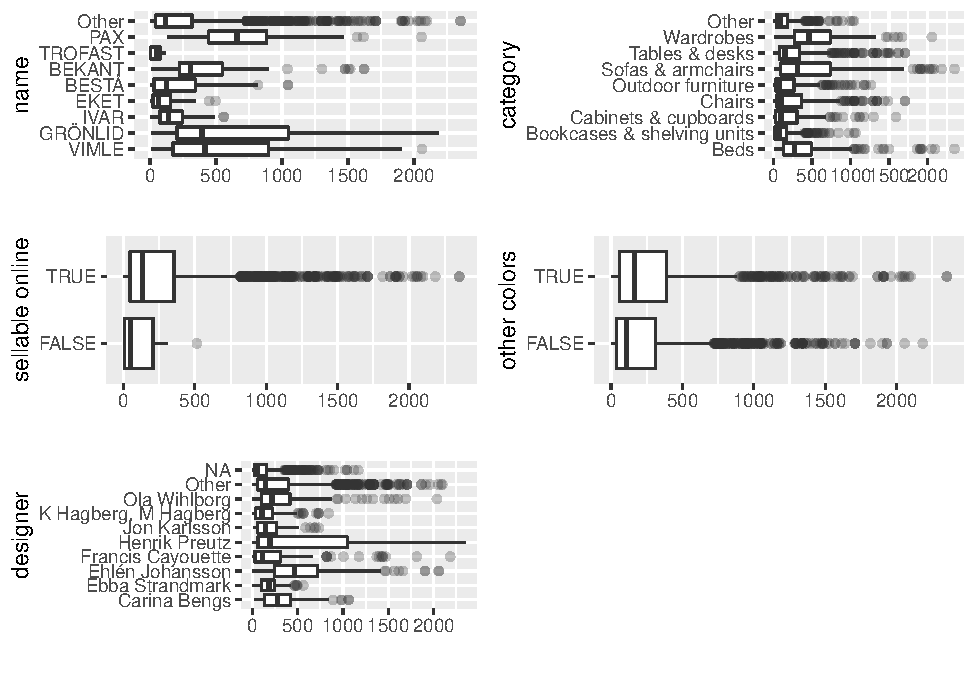
\includegraphics[width=1\linewidth]{_main_files/figure-latex/outliers-1} \caption{Boxplots for Price in € based on Independent Variables}\label{fig:outliers}
\end{figure}

\hypertarget{step-2-homogeneity-of-price}{%
\subsection{Step 2: Homogeneity of Price}\label{step-2-homogeneity-of-price}}

\textcolor{gray}{by P. Krück}

The homogeneity (homoscedasticity) of variance for price is explored by the means of conditional boxplotting.
Within each name, and within each category the variance is heterogenous (see fig. \ref{fig:homogeneity}). However, looking at both name and category in conjunction, it is possible to explore homoscedasticity of variance for price.

Due to the limited scope and length of this paper, the authors were not able to inspect all variable combinations for the three categorical plus two logical variables of the data set(\(2^5=32\)).

\begin{figure}
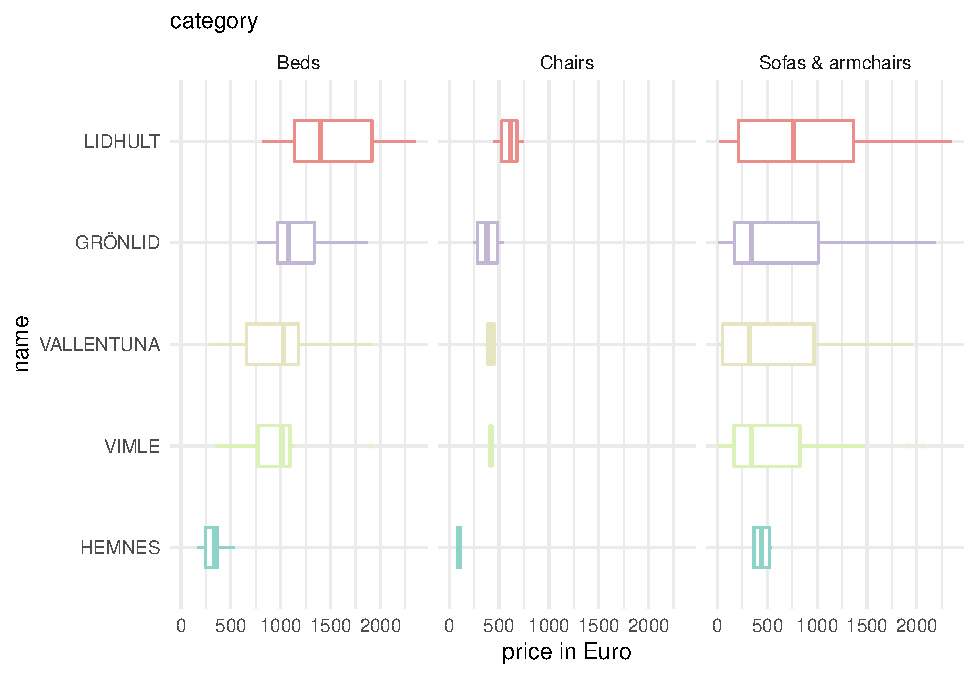
\includegraphics[width=1\linewidth]{_main_files/figure-latex/homogeneity-1} \caption{Homogeneity of category for selected combinations of name and category}\label{fig:homogeneity}
\end{figure}

\hypertarget{step-3-normality}{%
\subsection{Step 3: Normality}\label{step-3-normality}}

\textcolor{gray}{by P. Krück}

No numerical variables (\texttt{price}, \texttt{old\_price} and \texttt{size\_m3}) are arranged along a normal distribution (see fig. \ref{fig:normality}), but rather follow an exponential decay (\(e^{-x}\)).

\begin{figure}
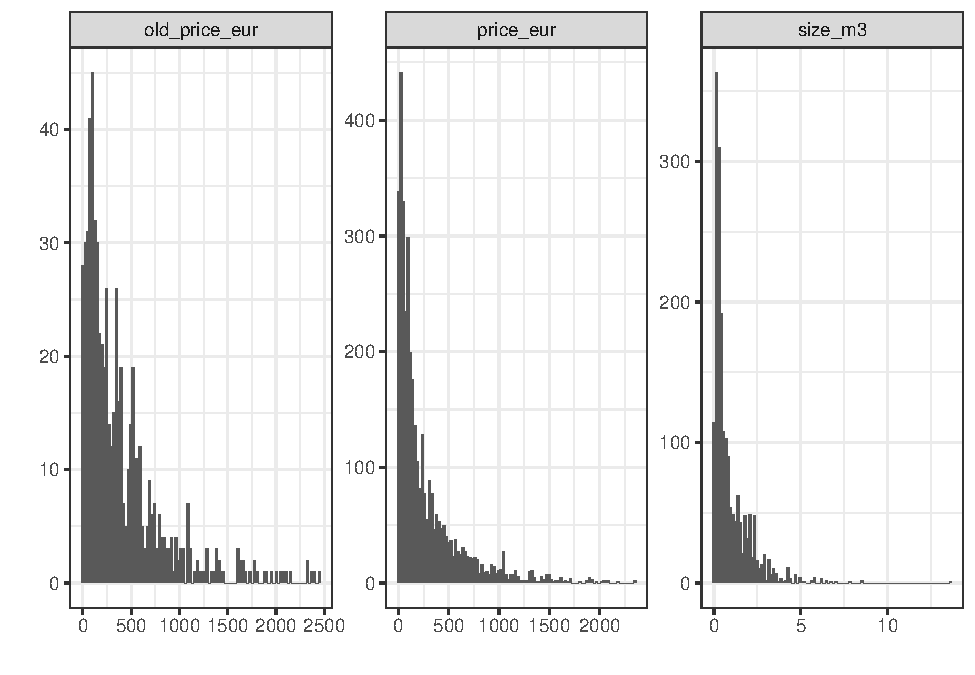
\includegraphics[width=1\linewidth]{_main_files/figure-latex/normality-1} \caption{Histogram of Numerical Variables with a Bin Width of 100 Euro}\label{fig:normality}
\end{figure}

\hypertarget{missing-values}{%
\subsection{Step 4: Missing Values}\label{missing-values}}

\textcolor{gray}{by P. Krück}

All variables were examined for missing values. Only \texttt{designer}, \texttt{size\_m3} and \texttt{old\_price\_eur} have missing values with percentages of 3.44\%, 45.9\% and 81\% respectively (see fig. \ref{fig:missing-values}).
The missing values for designer were deliberately set to \texttt{NA} by the authors in the case where the values contained digits, which is likely a scraping error.
The \texttt{NA} values for the size can be explained due to the computation of this column vector. \texttt{size\_m3} is the product of \texttt{depth}, \texttt{width} and \texttt{height}. If one of those three values is missing, the end result is also a missing value.
In contrast, the abscence of the old price variables is due to the fact that most items are not on sale and thus do not have a missing value.

\begin{figure}
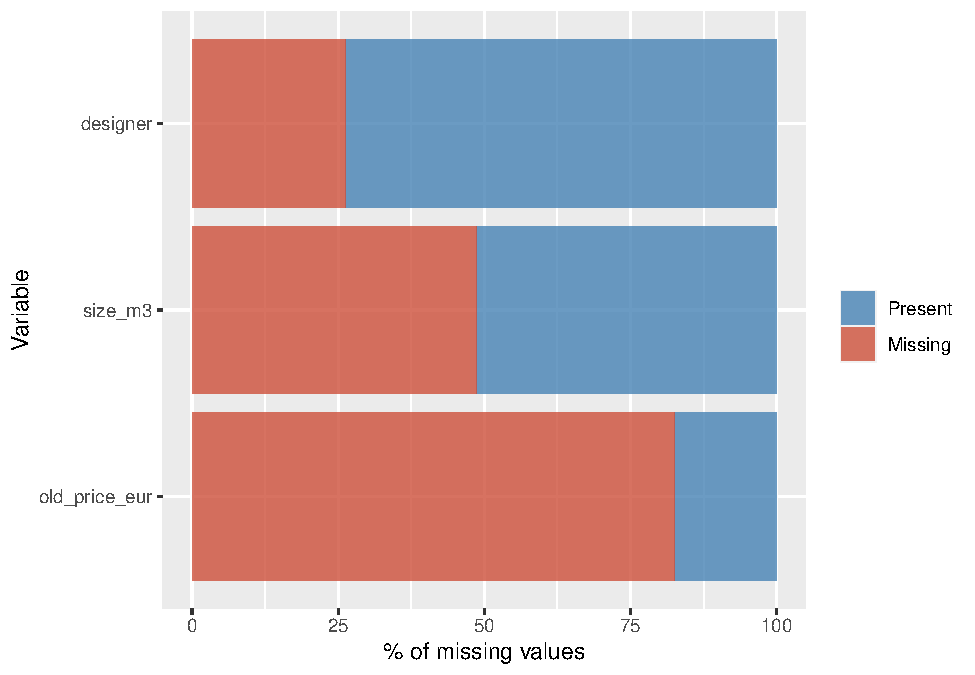
\includegraphics[width=1\linewidth]{_main_files/figure-latex/missing-values-1} \caption{Percentage of missing values}\label{fig:missing-values}
\end{figure}

\hypertarget{collinearity}{%
\subsection{Step 5: Collinearity between Independent Variables}\label{collinearity}}

\textcolor{gray}{by P. Krück}

The old price has a rather high variance inflation factor (VIF) which corresponds to high multicollinearity (see table \ref{tab:vif}). Contrarily, size has a low VIF which translates to low multicollinearity among the other independent variables (see table \ref{tab:vif}).

\begin{table}

\caption{\label{tab:vif}Variance Inflation Factors for Numerical Variables}
\centering
\begin{tabular}[t]{r|r|r}
\hline
price\_eur & old\_price\_eur & size\_m3\\
\hline
77.97 & 78.54 & 2.36\\
\hline
\end{tabular}
\end{table}

\hypertarget{relationship}{%
\subsection{Step 6: Relationship between Independent Variables and Price}\label{relationship}}

\textcolor{gray}{by P. Krück}

Inspecting the relationship between the independent variables and price, a strong correlation between \texttt{old\_price\_eur} and \texttt{size\_m3} can be observed, while none can be detected for the other variables (see \ref{fig:relationship-x-y}).
\texttt{old\_price\_eur} has a linear relationship (see fig. \ref{fig:relationship-old-price}) whereas \texttt{size\_m3} begins with a linear relationship as well, which is only disturbed by an outlier. (see fig. \ref{fig:relationship-size-m3}).

\begin{figure}
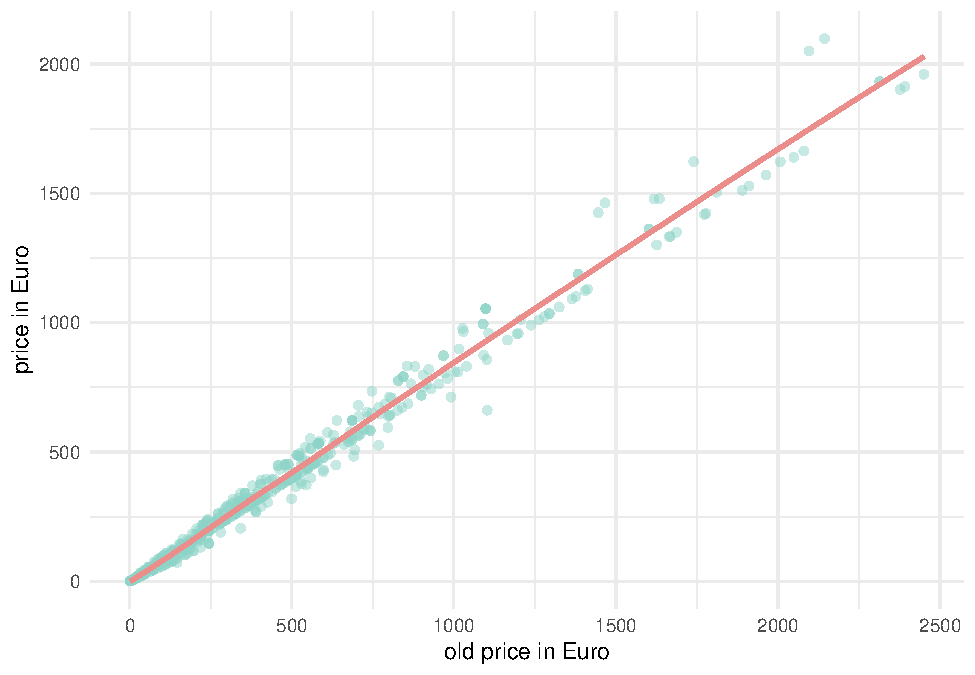
\includegraphics[width=1\linewidth]{_main_files/figure-latex/relationship-old-price-1} \caption{Relationshihp of Price and Old Price}\label{fig:relationship-old-price}
\end{figure}

\begin{figure}
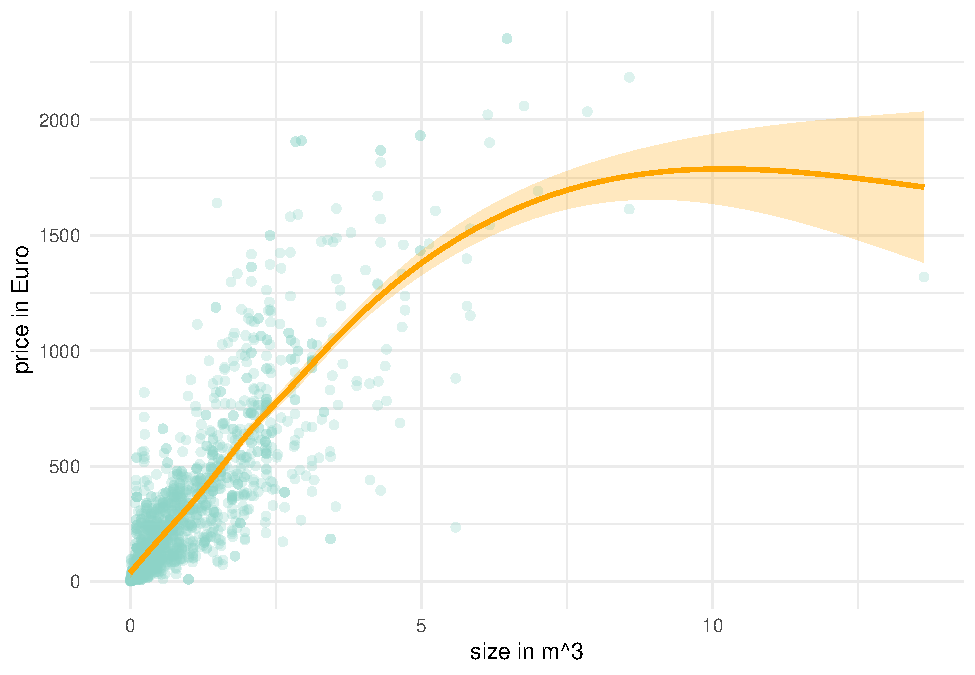
\includegraphics[width=1\linewidth]{_main_files/figure-latex/relationship-size-m3-1} \caption{Relationship of Price Size in Cubic Meters}\label{fig:relationship-size-m3}
\end{figure}

\hypertarget{step-7-interactions}{%
\subsection{Step 7: Interactions}\label{step-7-interactions}}

\textcolor{gray}{by P. Krück}

The interactions between different variables are explored by the use of conditioning plots (coplots).
Using this form plotting the relationship of two numerical variables is explored by creating a matrix of plots subdivided by two categorical variables.
In the given data set there are three numerical and three categorical variables which can be explored in this form of interaction. For the numerical variables, \texttt{old\_price\_eur} has such a strong relationship with \texttt{price} (see fig \ref{fig:relationship-old-price}). A more detailed breakdown by the categorical variables would not reveal new information. This leaves the exploration of \texttt{size\_m3} and \texttt{price\_eur} subdivided by designer, name and category resulting in (\({3 \choose 2} = 3\)) combinations of coplots.

\hypertarget{size-price-interaction}{%
\subsubsection{Interaction of size and price coplotted by designer and name}\label{size-price-interaction}}

\textcolor{gray}{by P. Krück}

It is unlikely that there is an interaction between size and price split by name and designer as is indicated by the non-parallelism of the fitted lines in the coplot (see figure \ref{coplot-code-designer-name}).

\hypertarget{problems-with-coplot-development}{%
\subsubsection{Problems with Coplot Development}\label{problems-with-coplot-development}}

\textcolor{gray}{by P. Krück}

This section describes a programming error the authors ran into regarding coplotting.

Unfortunately, the authors of this papers weren't able to fully explore all combinations.
Plotting designer and name works (see section \ref{size-price-interaction}) while the other two options would not plot properly.
The authors could not fully debug the problem with these plots.
The linear model predicted infinite values for some of the coplotted combinations for both amalgamations that wouldn't render correctly.
Dropping all \texttt{NA} values left 354 observations and the coplot would correctly render for the combination of \texttt{name} and \texttt{category} while for \texttt{name} and \texttt{designer} it would not. The number of observations for \texttt{name} and \texttt{category} is rather low considering the additional categorical subdivision which lead the authors to discard it as an insignificant research finding.
Still there seemed to be infinite values outputted by the linear method. The authors hypothesized that those values were caused by a division by 0 of the internal algorithm mechanics. This however proved to be wrong after applying the respective filters.
The code for the 3 plots can be viewed in Appendix chapter \ref{coplots}.

The inclined reader is encouraged to dabble with the code. Sending any hints or even a solution to fix the code and fully render the plots would be highly appreciated by the authors.\footnote{Any questions, hints or solutions may kindly be sent to philip.krueck@myhsba.de.}

\hypertarget{step-8-independence-observations-of-response-variable-price}{%
\subsection{Step 8: Independence Observations of Response Variable Price}\label{step-8-independence-observations-of-response-variable-price}}

\textcolor{gray}{by P. Krück}

The independence of observerations of the response variables assumes that ``{[}\ldots{}{]} information from any one observation should not provide information on another after the effects of other variables have been accounted for.''\footnote{Ibid., 11, ll.23--26.}
The data cleaning step left the observed data set in a tidy format which implies that the observations are independent of eachother.\footnote{``There are three interrelated rules which make a dataset tidy: Each variable must have its own column. Each observation must have its own row. Each value must have its own cell.'' (, Wickham, \emph{R for Data Science}, 149, ll.4--7.)}

\hypertarget{rf}{%
\section{Random Forest Regression Model}\label{rf}}

\textcolor{gray}{by J. Pein}

To analyze the feature importance of different variables on the price variable, a random forest model was chosen. In the given data set, categorical variables with lots of different values can be observed. Including all of those values in, for example, a linear regression model, would most likely lead to overfitting (see section \ref{overfitting}). This is because the linear model would learn the immanent data structure of the sample, but would not be able to generalize from this. Thus, the authors chose the random forest model, because according to Breiman\footnote{``Random Forests,'' 29.} it is robust against overfitting.

In this analysis, the R \emph{randomForest} package was used, which is based on the original Breiman and Cutler's Fortran code for random forest regression. To reproduce the results, the further data preparation steps are described here. These steps are based on the cleaned ikea data set which is described in section \ref{datacleaning}. This data set is then transformed further allowing it to be used with the \emph{randomForest} package. To learn more about how random forests work see chapter \ref{chapter-2}, to learn more about the \emph{randomForest} package see Liaw and Wiener.\footnote{``Classification and Regression by randomForest.''}

First, the variable \texttt{old\_price\_eur} is removed from the cleaned ikea data set, due to a very high correlation and relationship to the response variable \texttt{price\_eur} (price) analyzed in section \ref{collinearity} and section \ref{relationship}. Then, the \texttt{designers} and \texttt{names}, which are not part of the 50 \texttt{designers} and 49 \texttt{names} with the highest number of occurences, are grouped in the \texttt{other} value. This is because the \texttt{randomForest} method does not allow categorical variables with more than 53 predictors. The last step deals with the missing values in the data. As described in section \ref{missing-values}, there are many missing values in the \texttt{size\_m3} and \texttt{designer} variables. To apply the \texttt{randomForest} method of the \emph{randomForest} package on the data, those missing values are treated using three different approaches. In the first approach the rows with missing values are deleted, reducing the total number of rows by aproximately 50\%. In the second approach the missing values are dummy coded with a value of -1000. The third approach uses the \texttt{na.roughfix\ =\ na.omit} argument, which is the built-in way of the \emph{randomForest} package to deal with missing values.
After preparing the data, the \texttt{randomForest} method of the \emph{randomForest} package is applied to the data with number of trees set to 2000 and importance set to \texttt{TRUE}, training the random forest model with the prepared ikea data set.

\texttt{randomForest(price\_eur\ \textasciitilde{}\ .,\ rf\_ikea,\ ntree=2000,\ importance=TRUE)}

Then the \texttt{importance} method of the \emph{randomForest} package is used to calculate the feature importances, which are computed by permuting feature importance, which was introduced in section \ref{feature-importance}. The three different approaches of dealing with the missing values in the data set lead to different results, so the authors chose to calculate the mean result of the three approaches. The result of this analysis is presented in the following chapter.

\hypertarget{results}{%
\chapter{Results}\label{results}}

\hfill\textcolor{gray}{by J. Pein}

\hypertarget{todo-set-n_trees-to-2000-before-handing-in}{%
\section{TODO: set n\_trees to 2000 before handing in}\label{todo-set-n_trees-to-2000-before-handing-in}}

In this chapter, the result of the analysis of the feature importance of different features on the response variable price of Ikea products are presented.

As described in section \ref{rf}, the feature importance was calculated using permuting feature importance of the \emph{randomForest} R package. In this analysis, feature importance is derived from the percentage increase of the mean squared error (MSE) of the overall random forest regression model in regard to the response variable \texttt{price\_eur}. A larger percentage increase of the MSE implies greater feature importance. Conversely, a lower percentage increase of the MSE translates to less feature importance.

\begin{figure}
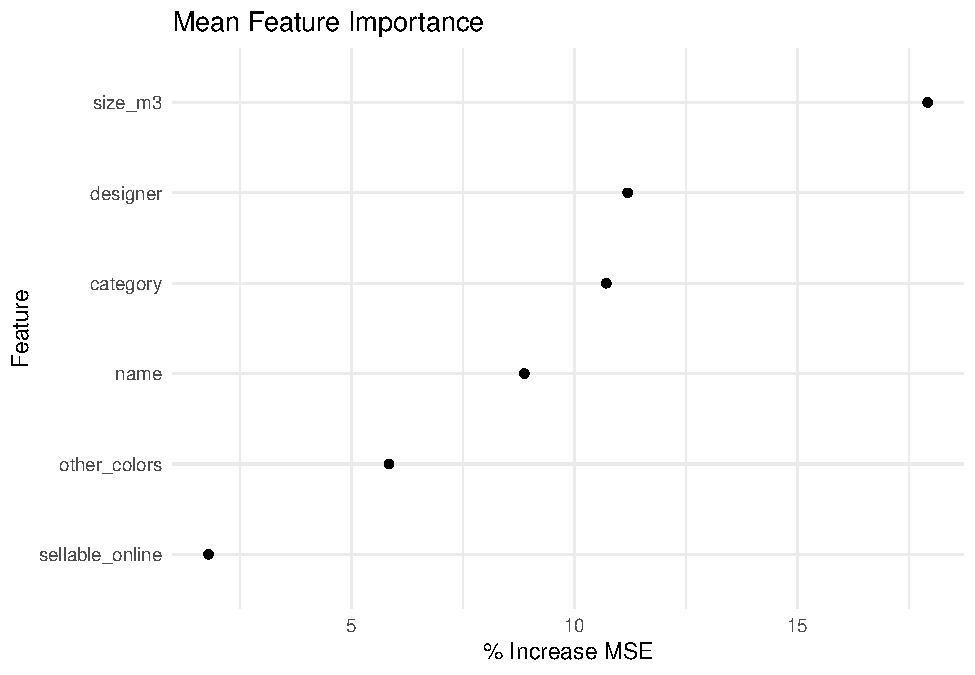
\includegraphics[width=1\linewidth]{_main_files/figure-latex/mean-feature-importance-1} \caption{A Plot Showing the Mean Feature Importance of the Predictor Variables on the Response Variable}\label{fig:mean-feature-importance}
\end{figure}

Thus, as can be seen in figure \ref{fig:mean-feature-importance}, the most important feature is \texttt{size\_m3} with an increase of the MSE of 182\%. The second, third and fourth most important features are \texttt{designer} with an MSE increase of 120\%, \texttt{name} with an increase of 114\% and \texttt{category} with an increase of 105\%. The fifth most important feature is \texttt{other\_colors} with a MSE increase of 78\% and the least important feature is \texttt{sellable\_online} with a 9\% increase.

These results are further discussed in the following chapter.

\hypertarget{discussion}{%
\chapter{Discussion}\label{discussion}}

\hfill\textcolor{gray}{by J. Pein}

In this chapter, the results are discussed in connection with the research question. The question that the results were supposed to answer is the following:

\emph{How important are the different features of Ikea products in regard to their price?}

\hypertarget{feature-importance-1}{%
\section{Feature Importance}\label{feature-importance-1}}

The \texttt{size\_m3} variable is the most important feature. Probably the main reason for this is the size of a product being closely linked to its material cost. Big items are generally more costly to produce, thus leading to a higher selling price and vice versa. Due to the high correlation to the price variable described in section \ref{collinearity} and section \ref{relationship}, it is worth discussing in future research whether or not to include this variable in a possible predictive analysis model .

The \texttt{designer} variable is the second most important feature. When looking at the price distribution per designer, in can be clearly seen that the interquartile range (IQR) of price varies for each designer. In addition, the IQR often is smaller than 300€, thus showing a tendency towards a certain price range, which might be the reason for the relatively high feature importance of the designer variable. For the plot, see figure \ref{fig:price-dist-per-designer}.

The \texttt{name} variable includes around 50 different product names with partly small numbers of occurences. But, as can be seen in figure \ref{fig:homogeneity}, certain product lines (names) tend to be more expensive than others. \emph{LIDTHULT}, for example, is the most expensive product line in each of the categories \emph{beds}, \emph{chairs} and \emph{sofas \& armchairs} while \emph{HEMNES} is on the lower end of the price scale. This behavior explains a relatively high feature importance of the \texttt{name} variable.

\texttt{Category} is another feature with a relatively high importance. One reason for this is the different category's price distributions showing a clear tendency towards certain price segments (see figure \ref{fig:price-dist-per-category}), i.e.~wardrobes and beds are generally more expensive than chairs.

The feature importance of \texttt{other\_colors} is the second lowest, but still considerable. This still relatively high feature importance might be due to the difference of the mean price and the relatively small IQR (see: figure \ref{fig:price-dist-other-colors}). On the other hand, there is a large overlapping area within the IQR in the two expressions of \texttt{other\_colors} possibly reducing the feature importance.

The very low feature importance of the \texttt{sellable\_online} variable is probably because the low number of occurences of a product being sellable online. Only around 0.6\% of the products are sellable online.

\hypertarget{conclusion}{%
\section{Conclusion}\label{conclusion}}

The data used in this paper was scraped from the Saudi Arabian Ikea website, thus this analysis mainly focusses on Ikea products in the Saudi Arabian market. To analyze the geographically independent feature importances, more data should be scraped from other international Ikea websites. The research question of this paper, \emph{How important are the different features of Ikea products in regard to their price?}, could thus not be answered for the global Ikea product market, but for the Saudi Arabian market only.

Also, in further research, the results presented on the feature importance of the predictor variables on the response variable price should be validated by other techniques than the random forest model used in this analysis to achieve unbiased results.

Furthermore, based on this analysis a predictive model could be developed which predicts the price of Ikea products in the Saudi Arabian Market based on the features analyzed. This could be used by Ikea internally to analyze if the price of their new product aligns with the prices of the currently available product or by market researchers.

Lastly, the authors were surprised by the high feature importances of the variables \texttt{designer} and \texttt{name} computed by the random forest model. Both variables have lots different values, suggesting an overfitting of the random forest model. This, however, is objected by scientific research.\footnote{Breiman, ``Random Forests,'' 29.}
Exploring what the reason behind the high feature importances of the variables \texttt{designer} and \texttt{name} and if they are due to overfitting of a random forest model should be analyzed in future research.
If the high feature importance of the variables truly is not due to overfitting, this example backs up the thesis of Grömping\footnote{``Variable Importance Assessment in Regression: Linear Regression versus Random Forest,'' 317.} that random forests are able to discover deeper patterns in the data. These patterns are beyond the discussion applied here, showing the power of random forests models.

\startappendices

\hypertarget{appendix}{%
\chapter{Appendix}\label{appendix}}

\begin{figure}
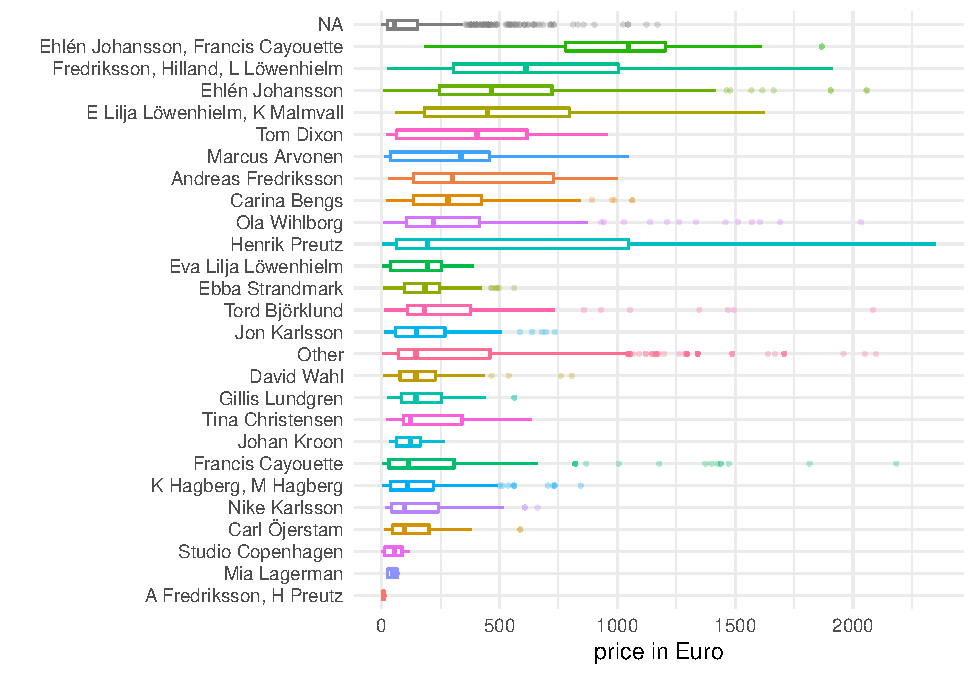
\includegraphics[width=1\linewidth]{_main_files/figure-latex/price-dist-per-designer-1} \caption{A Plot Showing the Price Distribution per Designer}\label{fig:price-dist-per-designer}
\end{figure}

\begin{figure}
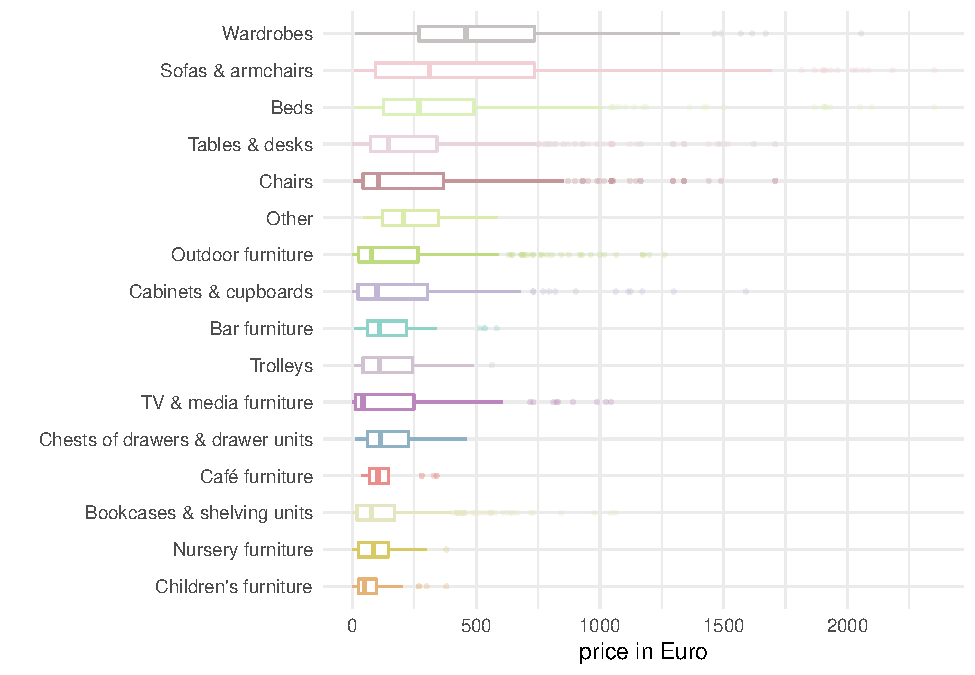
\includegraphics[width=1\linewidth]{_main_files/figure-latex/price-dist-per-category-1} \caption{A Plot Showing the Price Distribution per Category}\label{fig:price-dist-per-category}
\end{figure}

\begin{figure}
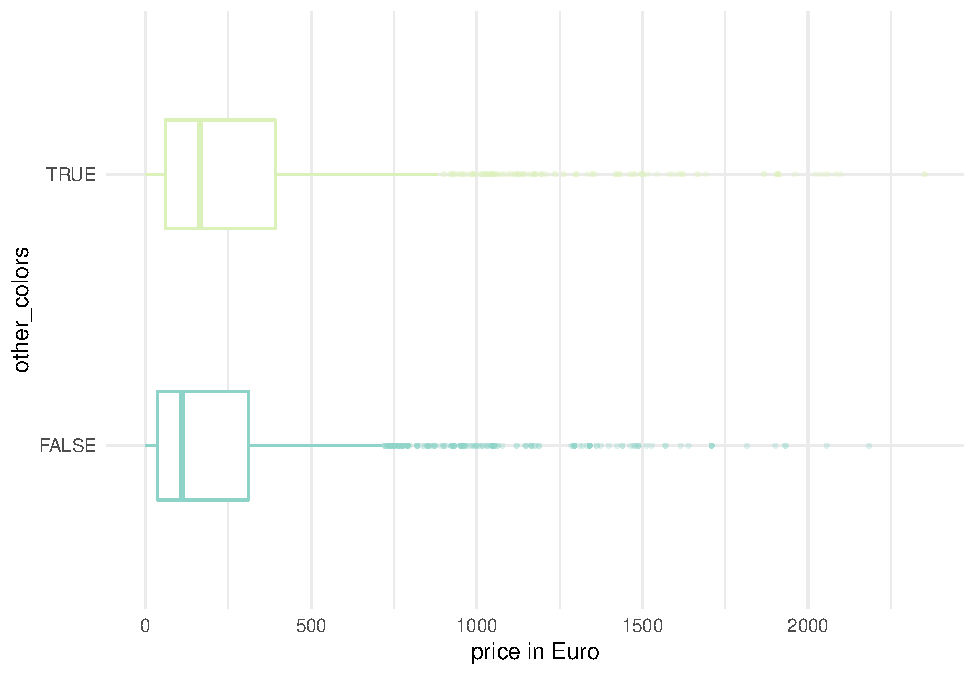
\includegraphics[width=1\linewidth]{_main_files/figure-latex/price-dist-other-colors-1} \caption{A Plot Showing the Price Distribution Other Colors}\label{fig:price-dist-other-colors}
\end{figure}

\begin{figure}[!h]
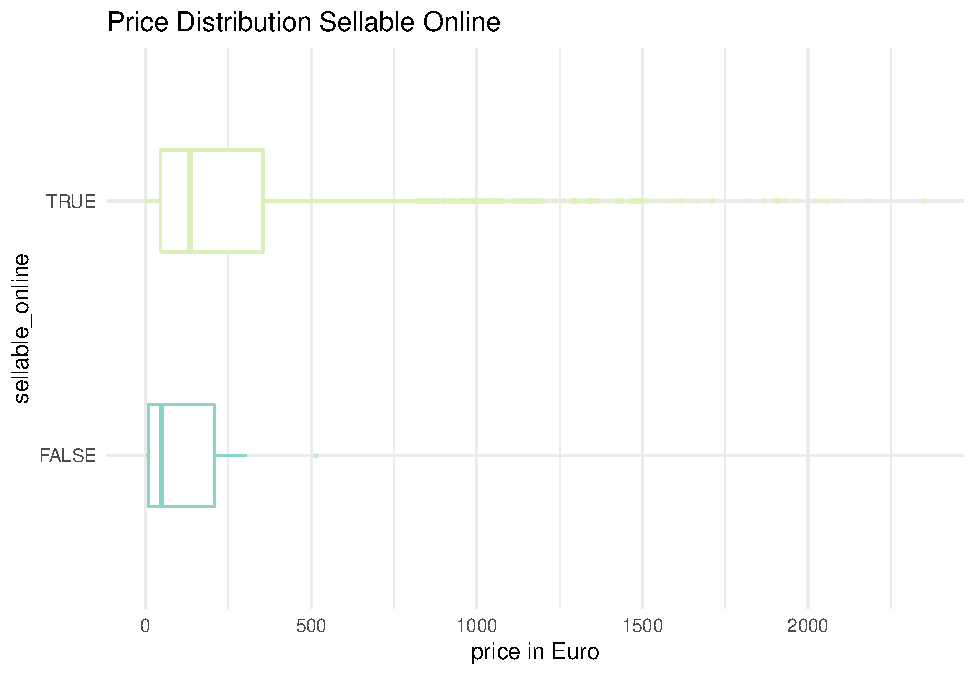
\includegraphics[width=1\linewidth]{_main_files/figure-latex/price-dist-sellable-online-1} \caption{A Plot Showing the Price Distribution Sellable Online}\label{fig:price-dist-sellable-online}
\end{figure}

\begin{figure}[!h]
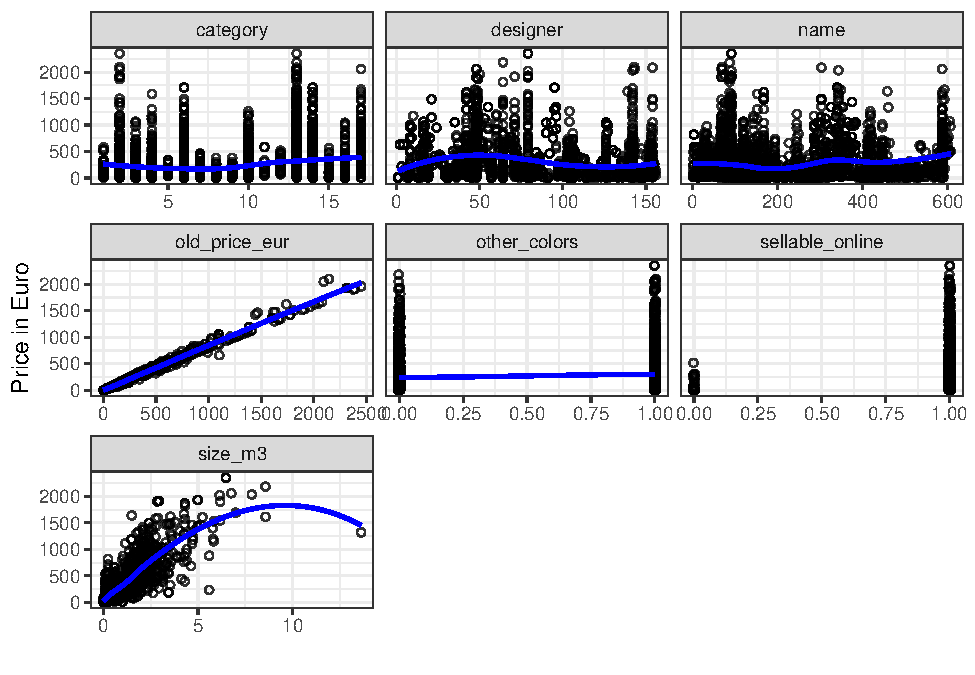
\includegraphics[width=1\linewidth]{_main_files/figure-latex/relationship-x-y-1} \caption{Relationship between Independent Variables and Price}\label{fig:relationship-x-y}
\end{figure}

\hypertarget{coplots}{%
\chapter{Coplots}\label{coplots}}

\begin{figure}[!h]
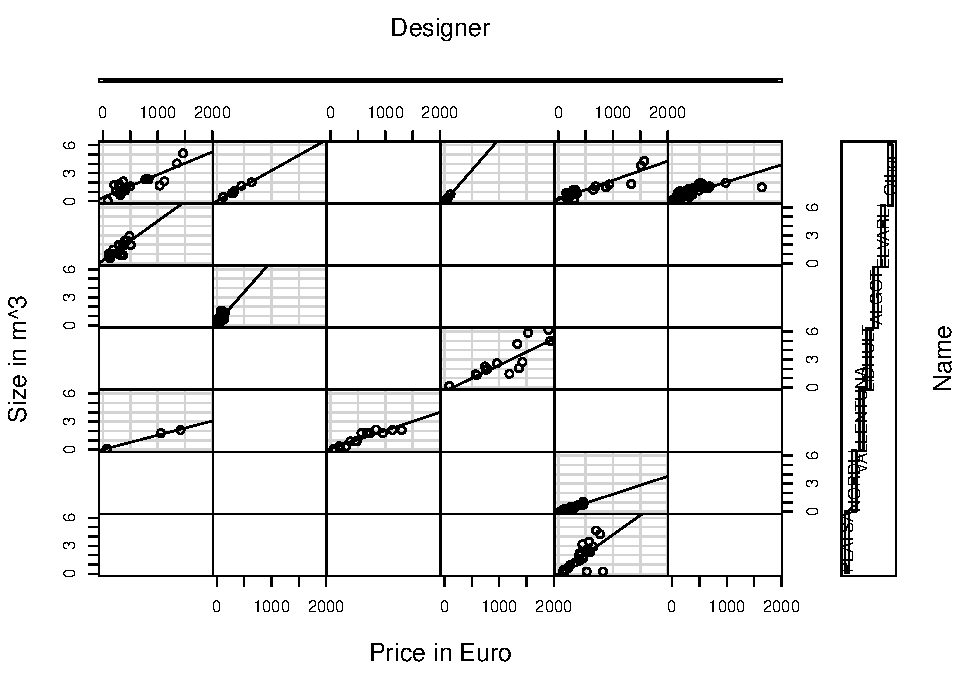
\includegraphics[width=1\linewidth]{_main_files/figure-latex/coplot-code-designer-name-1} \caption{Coplot of Size and Price Split by Designer and Name}\label{fig:coplot-code-designer-name}
\end{figure}

\begin{Shaded}
\begin{Highlighting}[]
\KeywordTok{coplot}\NormalTok{(size_m3 }\OperatorTok{~}\StringTok{ }\NormalTok{price_eur }\OperatorTok{|}\StringTok{ }\KeywordTok{fct_lump_n}\NormalTok{(category, }\DecValTok{5}\NormalTok{) }\OperatorTok{+}\StringTok{ }
\StringTok{         }\KeywordTok{fct_lump_n}\NormalTok{(name, }\DecValTok{5}\NormalTok{), }\DataTypeTok{data =} \KeywordTok{drop_na}\NormalTok{(tidy_ikea), }
       \DataTypeTok{ylab =} \StringTok{"Size in m^3"}\NormalTok{,}
       \DataTypeTok{xlab =} \StringTok{"Price in Euro"}\NormalTok{, }\DataTypeTok{panel =} \ControlFlowTok{function}\NormalTok{(x, y, ...) \{}
\NormalTok{         tmp <-}\StringTok{ }\KeywordTok{lm}\NormalTok{(y }\OperatorTok{~}\StringTok{ }\NormalTok{x, }\DataTypeTok{na.action =}\NormalTok{ na.omit)}
         \KeywordTok{abline}\NormalTok{(tmp)}
         \KeywordTok{points}\NormalTok{(x, y )\})}
\end{Highlighting}
\end{Shaded}

\begin{Shaded}
\begin{Highlighting}[]
\KeywordTok{coplot}\NormalTok{(size_m3 }\OperatorTok{~}\StringTok{ }\NormalTok{price_eur }\OperatorTok{|}\StringTok{ }\KeywordTok{fct_lump_n}\NormalTok{(designer, }\DecValTok{5}\NormalTok{) }\OperatorTok{+}\StringTok{ }
\StringTok{         }\KeywordTok{fct_lump_n}\NormalTok{(category, }\DecValTok{5}\NormalTok{), }\DataTypeTok{data =} \KeywordTok{drop_na}\NormalTok{(tidy_ikea), }
       \DataTypeTok{ylab =} \StringTok{"Size in m^3"}\NormalTok{,}
       \DataTypeTok{xlab =} \StringTok{"Price in Euro"}\NormalTok{, }\DataTypeTok{panel =} \ControlFlowTok{function}\NormalTok{(x, y, ...) \{}
\NormalTok{         tmp <-}\StringTok{ }\KeywordTok{lm}\NormalTok{(y }\OperatorTok{~}\StringTok{ }\NormalTok{x, }\DataTypeTok{na.action =}\NormalTok{ na.omit)}
         \KeywordTok{abline}\NormalTok{(tmp)}
         \KeywordTok{points}\NormalTok{(x, y )\})}
\end{Highlighting}
\end{Shaded}

\hypertarget{bibliography}{%
\chapter{Bibliography}\label{bibliography}}

\hypertarget{refs}{}
\leavevmode\hypertarget{ref-Breiman2001}{}%
Breiman, Leo. ``Random Forests.'' \emph{Machine Learning}, no. 45 (2001). \url{https://link.springer.com/content/pdf/10.1023/A:1010933404324.pdf}.

\leavevmode\hypertarget{ref-Groemping2009}{}%
Grömping, Ulrike. ``Variable Importance Assessment in Regression: Linear Regression versus Random Forest.'' \emph{The American Statistician}, nos. Vol. 63, No. 4 (2009): 308--19. \url{https://prof.beuth-hochschule.de/fileadmin/prof/groemp/downloads/tast_2E2009_2E08199.pdf}.

\leavevmode\hypertarget{ref-Liaw2002}{}%
Liaw, Andy, and Matthew Wiener. ``Classification and Regression by randomForest.'' \emph{R News}, nos. Vol. 2/3, December 2002 (2001). \url{https://www.researchgate.net/publication/228451484_Classification_and_Regression_by_RandomForest}.

\leavevmode\hypertarget{ref-Hadley2017}{}%
Wickham. \emph{R for Data Science}. O'Reilly Media, 2017.

\leavevmode\hypertarget{ref-Zuur2010}{}%
Zuur. ``A protocol for data exploration to avoid common statistical problems.'' \emph{British Ecological Society}, 2010. doi:\href{https://doi.org/10.1145/1738826.1738829}{10.1145/1738826.1738829}.


%%%%% REFERENCES

% JEM: Quote for the top of references (just like a chapter quote if you're using them).  Comment to skip.
% \begin{savequote}[8cm]
% The first kind of intellectual and artistic personality belongs to the hedgehogs, the second to the foxes \dots
%   \qauthor{--- Sir Isaiah Berlin \cite{berlin_hedgehog_2013}}
% \end{savequote}

\setlength{\baselineskip}{0pt} % JEM: Single-space References

{\renewcommand*\MakeUppercase[1]{#1}%
\printbibliography[heading=bibintoc,title={\bibtitle}]}

\end{document}
